\documentclass[preprint,3p, 11pt,authoryear]{elsarticle}


\usepackage{graphicx}
\graphicspath{{./Graphic/}}
\usepackage{array}
\usepackage{amssymb} % various useful mathematical symbols
\usepackage{gensymb} % for `degree' sign
\usepackage{amsthm}  % extended theorem environments
\usepackage{lineno}   % for line numbers
\usepackage{tabularx} % for adjustable table width
\usepackage[hidelinks]{hyperref}  % for hyperlinks
\usepackage{amsmath}
\newtheorem{property}{Property}[section]
\usepackage{soul}
\usepackage{epsfig}
\usepackage{tabularx}
\usepackage{multirow} 
\usepackage{setspace}
\usepackage{adjustbox}
\usepackage{xcolor}
\usepackage[utf8]{inputenc}
\usepackage{mathrsfs}

\journal{Nondestructive Testing and Evaluation}

\begin{document}

\begin{frontmatter}



\title{A methodology for calculating active force-time functions from broadband piezoelectric sensors}

 \author[1]{Paul A. Selvadurai \corref{cor1}}
 \ead{paul.selvadurai@sed.ethz.ch}
\author[2]{Rui Wu}
\author[3]{Claudio Madonna}
\author[2]{Omid Moradian}




\cortext[cor1]{Corresponding author, Post-Doctoral fellow}
\address[1]{Swiss Seismological Service, ETH Zurich, Zurich, Switzerland}
\address[2]{Engineering Geology Group, ETH Zurich, Zurich, Switzerland}
\address[3]{Department of Earth Sciences, ETH Zurich, Zurich, Switzerland}


\begin{abstract}
We preform active source tests using a piezoelectric (PZT) actuator that was excited by a rapid transient high voltage pulse (HVP). The crystal geometry of the actuator was a conical frustum where the tip was placed centrally on top of a thick steel plate. We studied the elastodynamic stress waves  (between 100 kHz to 1 MHz) produced by the source, whereby the HVP pulse was converted to a rapid transient force-time function ($f_{j}$) via the piezoelectric effect.  The source produced mechanical vibrations ($u_{k}$) throughout the sample and was measured ($s$) using an array of 13 passive conical PZT receivers, at known locations on the bottom of the steel plate. Dynamic Green's functions ($G_{kj}$) were calculated using generalized ray theory and the known instrument responses ($I_{k}$) were pre-calculated from a series of ball drop experiments for all source-receiver pairs. Using these parameters, we were able to reconstruct the force-time function of the PZT actuator. As predicted from the literature, the actuator behaved as an under-damped oscillator with a peak loads, decay rate and undamped resonant frequency of $A_{0}$ = 4.7 $\pm$ 0.8 N, $\Gamma$ = 0.7 MHz and $\Lambda$ = 4.7 MHz, respectively.  Both the decay rate and resonant frequency were determined as by minimizing the error between theoretical displacements for this force-time function over all 13 receiver measurements. Understanding calibrated force-time functions from PZT actuators can help to develop time-dependent and nondestructive characterization of many acoustic emission system components, such as the receiving transducers or the transfer media itself, in non-accessible laboratory environments. 
\end{abstract}

\begin{keyword}
Laboratory seismology, acoustic emissions,  piezoelectric sensors, absolute source calibration, 
\end{keyword}
\end{frontmatter}

\doublespacing
\linenumbers
\clearpage
%%%%%%%%%%%%%%%%%%%%%%%%%%%%%%%%%%%%%%%%%%%%%%%%%%%%%%%%%%%%%%%%%%%%%%%%%%%%%%%%%%%%%%%%%%%%%%%%%%%%%%%%%%%%%%%%%%%%%%%%%%%%%
\section{Introduction}
\label{int}

Understanding the theory associated with elastodynamic wave propagation in materials has proven to be highly applicable to many disciplines in science and engineering. The general principle follows that by measuring the kinematic motion at a point in/on the media as its perturbed by the incoming elastic waves, we can use wave propagation theory to back calculate critical information of the problem. The particle motions within the body are governed by the wave equation and the body itself can be a solid or fluid materials. The waves carry both information of the media in which they propagate and of the source which caused them. This concept has made for many practical and highly interdisciplinary applications. It has been widely applied in the fields of seismology, biomedicine, and nondestructive testing, to name a few.

The concept relies heavily on understanding attributes to three key components: (\textit{i}) source, (\textit{ii}) material and (\textit{iii}) receiver as shown in Figure \ref{fig2}. In most applications, these waves are non-intrusive, propagating elastically through the medium from the source to receiver. From this, the problem benefits from \textit{source-receiver reciprocity} and due to symmetry of the wave equation, \textit{time invariance} applies, making this a versatile and flexible problem.  

Sources can occur due to anthropogenic forcing, for example, rock samples subjected to outside stresses in a laboratory setting can crack locally, generating acoustic emissions \citep[e.g.][]{Lei2014, Moradian2016}. These emission cause vibrations within sample and these are recorded using peizoelectric sensors at known locations. This phenomena also scales up to mining activities where microseismic studies are performed to ensure safety during engineering activities \citep[e.g.][]{Manthei2018}. Further up the scale, large natural earthquakes on faults are activated by slow tectonic loading on geologic timescale. At each scale, the physic governing wave propagation holds and the vibrations through the medium are studied with arrays of sensors that are sensitive to vibrations at a range of frequencies. When the sources occur due to spontaneous instability, we consider this to be passive monitoring.

Sources can also be actively imposed, meaning that a transient force must manufactured within or on the body of interest. Since the wave equation still governs the motions throughout the body, it becomes an important tool to study the material properties or changes in them over time. Moreover, if multiple sources can be manufactured at varied locations, it becomes possible to understand structures through, for example, tomographic inversion.  This has been particularly important in the medical industry, where ultrasonic sensors can act as source or receivers and structures within the subject can be non-invasively reconstructed through ultrasound computer tomography (USCT) \citep[e.g.][]{Christensen1988}. While medical applications assume that acoustic waves propagate (i.e. fluid), \textit{active field surveys} in geophysics assume that the material is a solid and can reconstruct the subsurface to a high degree of certainty using `shot gather' approach and having well-constrained and repeatable sources.

In this study, we aim to study properties of ab active source produced in a controlled laboratory setting. Active survey in the laboratory have been employed for decades and typically study vibrations in the range of 100 kHz to 5 MHz. Many source can be manufactured from pencil lead fracture, capillary fracture, capacitive transducer, conical transducer, ball impact, spark, and high explosive \citep{Breckenridge1990}. As stated above, understanding attributes of the source is paramount to gaining more insight of the material it samples with the elastic waves. We aim to better understand the exact nature of the transient force produced when a rapid voltage transient is applied to a conical piezoelectric actuator. However, since direct measurement of this force is not easy at the frequencies required, we aim to infer the force-time function by studying the ground motions on an array of passive sensors. To simplify the problem we study the wave propagation problem in a homogeneous and elastic material.

\subsection{Lamb's problem and PZT actuators}

The study of waves in an elastic half-space was solved by \citet{Lamb1904} who was interested in the kinematic motions on a surface using the integral of plane waves solutions from \citet{Rayleigh1885}. More specifically, the Lamb's problem focuses on determining the elastic disturbance resulting from a point force in/on a half space. These early studies aimed to understand wave phase arrivals and their relationship to earthquake sources in the field of seismology. These seminal investigations have been followed by many hundreds of studies that have use different mathematical approaches to solve the wave equation \citep[e.g. ch 6 in][]{Aki2002}. These studies vary in complexity, for example in the media (in-homogeneous layered, or anisotropic, etc.), with the sources (double couple, compensated-linear-vector-dipole, etc.) and use a range of different methods to solve (theoretical closed-form solutions, numerical methods, etc.). We adopt the approach presented by \citet{Johnson1974} that derived the complete solution to the three-dimensional Lamb’s problem derived using the Cagniard--de Hoop method. This solution is used to study the mechanical disturbances from sources in an elastic half-space and has been implemented in a numerical generalized ray theory code by \citet{Hsu1985} \citep[see also][]{McLaskey2011, McLaskey2012, Selvadurai2019}.

While more complex sources have been considered to model earthquakes, such as the single and double couple source, we believe the original problem studied by \citet{Lamb1904} -- elastic displacements resulting from a point force in/on a half space -- is sufficiently complex for capturing the behavior of the piezoelectric actuator depicted in Figure \ref{fig2}(a). In Figure \ref{fig2}(a), we show the cross-section of the problem at hand. The source is produced by pulsing the piezoelectric actuator on the top surface using the experimental facilities described in Section \ref{ExpFac}. The impulsive actuation of the PZT crystal on the steel plate produces a rapid transient source causing elastodynamic stress waves to propagate outwards. In Figure \ref{fig2}, the coloured region represents a synthetic representation of the velocity wave-field and is only provided as a reference and is not representative of the wave-field we study here. This snapshot of the velocity wave-field represents that produced from a capillary fracture and was solved using a numerical finite element approach in ABAQUS \citep[adapted from fig. 2][]{Selvadurai2019}. 

Properties of the source creating the stress waves is important. \citet{Breckenridge1990} states that the ideal source is infinitesimal in size, has a force-time function of a step or delta function, and generates large amplitudes. He performed important study of a variety of sources including pencil lead fracture, capillary fracture, capacitive transducer, conical transducer, ball impact, spark, and high explosive. He noted that each type is imperfect and has its trade offs. In this study, we look to aim to understand the PZT actuator (similar their conical transducer) which we can be leverage to non-invasively study the \textit{in situ} conditions inside less accessible experimental facility (e.g. triaxial pressure cell). To model the force-time function produced conical sensor, we first simplify the sequence of events and their components that link the source to the recorded signal.

In Figure \ref{fig2}, we show the five components of ``toolchain'' that is used to link the source to the measured signal and governed by the wave equation. The PZT actuator is used to produce (\textit{1}) a \textbf{rapid transient force} $f_{j}$ on the top surface at a point $\mathbf{\xi}$ of the steel platen at a delayed time $\tau$. Elastic stress waves propagate through the plate and the theoretical elastic displacement field throughout the body can be solved for using (\textit{2}) \textbf{Green's function} $G_{kj}$. The Green's functions map the (\textit{3}) \textbf{mechanical vibrations} $u_{k}$ at point $\mathbf{x}$ and time $t$ to the force at point $\mathbf{\xi}$ and time $\tau$. A passive sensor on the bottom surface at point $\mathbf{x}$ attempts to measure the theoretical displacements $u_{k}$. Unfortunately, all passive sensors distort the (\textit{4}) \textbf{measured signal}  $s$.  This distortion can be quantified according to its (\textit{5}) \textbf{instrument response} $i_{k}$. 

\begin{figure}[h]
     	\centering
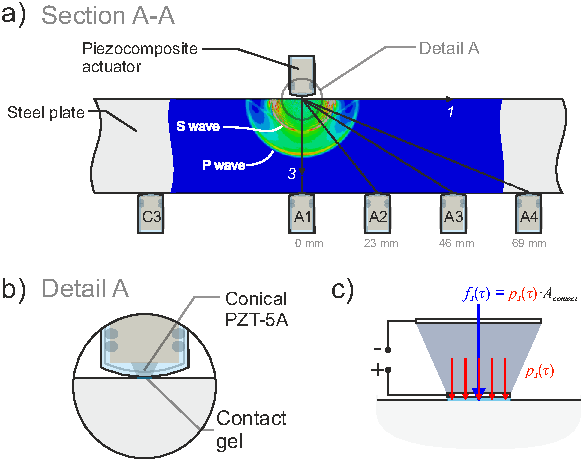
\includegraphics[scale= 1.0]{FIG2.pdf} 
\caption{Fundamental features related to the Lamb problem that relates elastodynamic displacements in an elastic half-space to a source (force-time) function. The velocity field is shown for reference only and was adopted from \citet{Selvadurai2019}. P and S waves are highlighted for reference only. The PZT actuator is located centrally on the top of the steel plate and passive (recording) sensors are shown below for the Section A-A from Figure \ref{fig1}(b).}
	\label{fig2} 
\end{figure}
\section{Experimental facilities}
\label{ExpFac}
\subsection{General}

We study elastodynamic waves propagating through an elastic isotropic, homogeneous steel plate. Using an electro-mechanical piezoelectric actuator, we deliver an impulsive transient source to the top surface of the steel specimen. An array of 13 piezoelectric (lead zirconate titanate, PZT) transducers are mounted on the  in an aluminium array holder. The aim of this study is to better understand the force produced by the piezoelectric actuator by studying the waves produced at different locations on the bottom of the specimen.

\begin{figure}[ht]
     	\centering
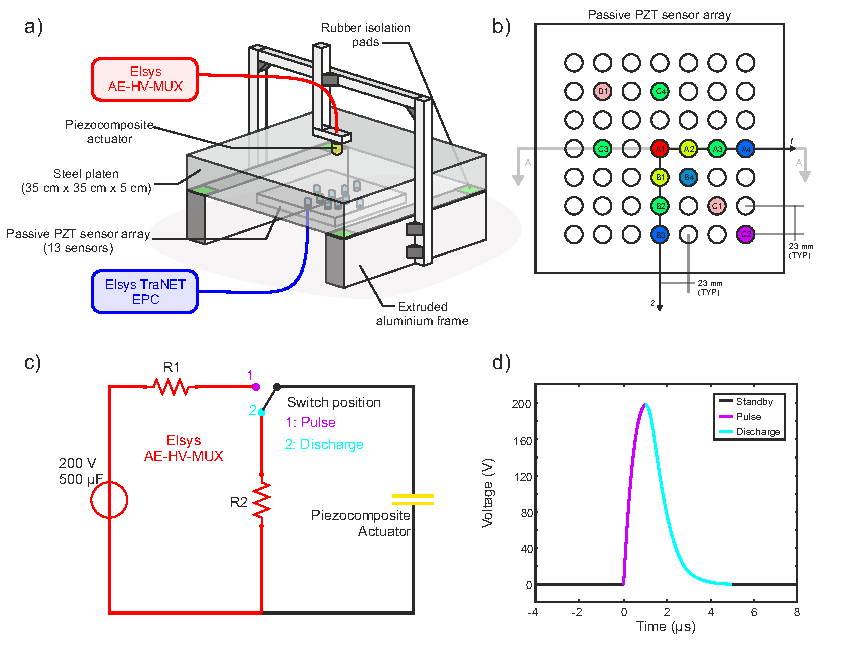
\includegraphics[scale= 1.0]{FIG1.pdf} 
\caption{\textbf{(a)} General schematic of the sensor calibration station at the Rock Physics and Mechanics Laboratory at ETH Zurich. We use this apparatus to apply an active source downwards using a PZT actuator located centrally on the top of a steel plate. This produced elastodynamic stress waves that are measured using an array of 13 broadband, passive PZT sensors on the bottom of the plate. \textbf{(b)} The array of passive PZT sensors are shown where the colors indicate their epicentral location with respect to the source and these colors used throughout the study. \textbf{(c)} The driver circuit for voltage pulse that shows the elements associated with the Elsys high-voltage pulsing unit (AE-HV-MUX). \textbf{(d)} The solution for the time-dependent voltage pulse and discharge applied across the PZT element. }
	\label{fig1} 
\end{figure}

Figure \ref{fig1}(a) shows a schematic representations of the steel platen (350 mm $\times$ 350 mm $\times$ 50 mm) in the extruded aluminium frame. Small rubber pads (5 mm $\times$ 5 mm $\times$ 1 mm) are used to base isolate the steel platen from the frame. Material properties of the steel plate required to model the wave propagation problem are given in Table \ref{table1}. Centrally located on the top surface is a piezoelectric actuator built in-house.  This sensor is connected to an high-voltage pulsing unit (HVP, Elsys Instruments AE-HV-MUX). This unit consist of a PiezosystemJena voltage amplifier for pulse generation (HVP 1000/200) that is fully integrated with the data acquisition (DAQ) software (Elsys Instruments TraNET). Figure \ref{fig1}(c) shows the circuit diagram of the HPV that is used to deliver an amplified voltage pulse to the piezoelectric actuator. The pulse and discharge of the system is depicted in the Figure \ref{fig1}(d). The time-dependent change in voltage when the switch position is in ``pulse'' (state 1) is given as:

\begin{equation}
\begin{array}{lcc}
  V(t) =  V_{0} \cdot \left[ 1 - exp\left(\frac{t}{R_{1}\cdot C_{PZT}} \right) \right], & \text{for} & 0 < t \leq t_{0}\\
\end{array}
\label{eq1}
\end{equation}

\noindent where $C_{PZT}$ = 300 pF, $R_{1}$ = 5 $\Omega$, $V_{0}$ = 200 V and the time of the pulse was set to $t_{0}$ = 1 $\mu$s. Discharging the systems required the switch to move to position 2 and we can solve for the theoretical discharge voltage:

\begin{equation}
\begin{array}{lclcc}
  V(t) =  V_{0} \cdot exp\left(-\frac{t - t_{0}}{R_{2}\cdot C_{eq}}\right), & \text{for} & t > t_{0}\\
\end{array}
\label{eq2}
\end{equation}

\noindent where $R_{2}$ = 1000 $\Omega$, $C_{eq}$ is the equivalent capacitance of $C_{PZT}$ and $C_{0}$ in series using electrostatic theory.  

Figure \ref{fig1}(b) show the array holder for the passive PZT sensor (KRN Services model: KRNBB-PC) which are used to measure the stress waves produced by the active piezoelectric source. The aluminium array had a 7 $\times$ 7 locations with 23 mm spacing in both the $1$- and $2$-directions.  In this study, we have assumed our source is symmetric about the $1-3$ and $2-3$ planes (i.e. aligned in the $3$-direction) and, therefore, have focused most of our passive sensors converge to one quadrant of the array holder.  Similar colors of the sensors locations in Figure \ref{fig1}(b), represents their epicentral locations.  We have redundant measurements at all epicentral locations expect $x$ = 0 mm, 33 mm and 96 mm and we show in Section \ref{results} that there appears to be little to no misalignment of the active source.  

A total of 13 sensor are used and the spectral characteristics of these sensors have been well examined in the literature using the absolute calibration methods \citep{Glaser1998, McLaskey2010, McLaskey2012, Selvadurai2015, Selvadurai2019, Wu}. \citet{Glaser1998} provides a detailed account to sensor attributes. This sensor includes a the small field emission transistor (FET)-based (Sanyo model: 2SK715W) that preamplifies internally to improve impedance matching and loss due to wire capacitance.  These sensors have shown flat displacements-responses between 100 kHz to 1 MHz \citep{McLaskey2012, Selvadurai2019}.  At longer wavelengths between 1 kHz to 50 kHz these sensors have been found to behave more similar to an accelerometer \citep{Wu}.

\begin{table}[ht]
	\centering
	\caption{Material properties of HABA CK45 steel test platen.}
	\begin{tabular}{ m{5cm} m{2cm} m{4cm}} 
		\hline  
		\bf{Parameter} 			& \bf{Symbol} 		& \bf{Value}	\\
	    Density                 	& $\rho$            & 7850 kg/m$^{3}$\\
	    Shear modulus        & $\mu$             & 84 GPa \\
	    Poisson's ratio         & $\nu$             & 0.28\\
	    P wave velocity       & $V_{P}$           & 5890 m/s\\
	    S wave velocity       & $V_{S}$           & 3270 m/s\\	    
		\hline  	
	\end{tabular}
	\label{table1}
\end{table}

\section{Theoretical Framework}
\label{theo}

We build on the recent studies of signal analysis and instrument calibration by \citet{McLaskey2012} and continuing our analysis using Green's function formalization \citep{Aki2002, Johnson1974}. Due to spatial reciprocity of the representation theorem \citep{Aki2002} and the invariant nature of the seismic wave equation to time-reversed solutions \citep{Fink1992}, we can use convolution of the components highlighted in Figure \ref{fig2} to analyze our linear time-invariant (LTI) system. This approach assumes that changes in the sensor and source behavior and material properties are unaffected over time.  We assume point representations at both the sensor and source location, which might be influenced so-called ``aperture'' effect. However, this is minimized by using a smaller contact point characteristic of the conical frustum PZT crystal, which will be discussed later when we examine in more detail how the force systems of the PZT actuator.

Using the classical theory describing dynamic elasticity \citep{Aki2002}, we use Green's functions to relate the displacement $u$ at a known location $\mathbf{x}$ and time $t$ to a force $f$ at another point $\mathbf{\xi}$ and time $\tau$. This is given as the convolution of the force with the Green's function

\begin{equation}
\label{eq1}
           u_{k}\left( \mathbf{x}, t \right)  =  
            f_{j}\left( \mathbf{\xi}, \tau \right) \ast 
            g_{kj}\left( \mathbf{x}, t;\mathbf{\xi}, \tau \right).
\end{equation}

\noindent We note that $\ast$ represents convolution in the time domain, subscripts reflect Einstein summation convention, $f$ is the force acting in the $j$ direction at location $\mathbf{\xi}$ and $g_{kj}\left( \mathbf{x}, t;\mathbf{\xi}, \tau \right)$ is the elastodynamic Green's function describing the displacement $u$ in the direction $k$ at location $\mathbf{x}$. For the elastodynamic solutions studied here, we assume that convolution $\ast$ is applicable since the system in question are linear time-invariant (LTI) and that convolution has commutativity, associative and distributive properties. The true Green's function is the displacement field for the unit impulse force $\delta_{j}$ or the identity convolution. 

Piezoelectric transducers measure a voltage caused by the compression of the lead zirconate titanate (PZT) crystal in the surface normal direction $s\left( \mathbf{x}, t \right)$. We can relate the true surface displacement $u_{k}$ to voltage measurement $s$ using the instrument response, which is given as
   \begin{equation}
    \label{eq2}
        s\left( \mathbf{x}, t \right) =
            u_{k}\left( \mathbf{x}, t \right) \ast i_{k}\left(\mathbf{x},t \right).
    \end{equation}
    
    \noindent Combining \eqref{eq1} and \eqref{eq2}, we can represent the measured voltage to the forces which produced them:

    \begin{equation}
    \label{eq3}
        s\left( \mathbf{x}, t \right) =
            u_{k}\left( \mathbf{x}, t \right) \ast i_{k}\left(\mathbf{x}, t \right) =  
                f_{j}\left( \mathbf{\xi}, \tau \right) \ast 
                g_{kj}\left( \mathbf{x}, t;\mathbf{\xi}, \tau \right) \ast i_{k}\left(\mathbf{x},  t \right).
    \end{equation}

\noindent We can also use this formulation to relate the measured signals to a set of self-equilibrating forces or moments $m_{jp}$ \citep{Aki2002}. Displacements in the body are related to the spatial derivative of the elastodynamic Green's function $g_{kj,p}$.  While this is more similar to sources buried within a specimen and may be more representative of an earthquake source, this is not the focus of this study.  In this study, all sources are produced on the surface of the specimen, which justifies the use of only equation \eqref{eq2}.

\subsection{Time Domain Characteristics of the Force-Time Function}
\label{force_time}

Our study aims at determining the nature of the dynamic transient source produced from the PZT actuator. We first decompose the source into two parts as shown here:

\begin{equation}
    \label{eq4}
    f_{j}\left( \mathbf{\xi}, \tau \right) =A_{0} \cdot f^{*}_{j}\left( \mathbf{\xi}, \tau \right) ,
\end{equation}

\noindent where $f^{*}_{j}$ is the normalized force-time function that has units (N) and a general shape to that follows the electro-mechanical behavior of the coupled high-voltage discharge and sensor systems.  A unitless scaling factor $\kappa(\tau)$ will be used to scale the normalized force time-function $f^{*}$ to the true force-time function $f$ and likely varies with the time as the electrical pulse is applied to the active source.

\begin{figure}[ht]
     	\centering
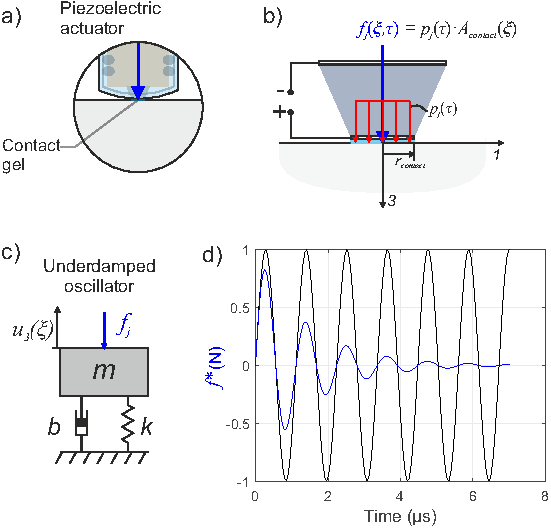
\includegraphics[scale= 0.9]{FIG2b.pdf} 
\caption{\textbf{(a)} Enhanced view of the contact region from the concial PZT actuator. \textbf{(b)} Simplified schematic showing the electro-mechanical systems and the estimate region where a pressure pulse $p_{j}$ (red) is generated when excited by the impulsive voltage. We assume that the force-time $f_{j}$ (blue arrow) is simply the integration of transient pressure over a constant circular contact area $A_{contact}$ and acting only in the 3-direction.  \textbf{(c)} Model summarizing the complex behavior of the PZT actuator (both internal and external) using an under-damped spring-mass damper systems whose behavior follow equation \eqref{eq4b}. \textbf{(d)} The normalized force-time function for: $A_{0}$ = 1 N, $\Gamma$ = 0 MHz and $\Lambda$ = 4.7 MHz (black line) and $A_{0}$ = 1 N, $\Gamma$ = 0.7 MHz and $\Lambda$ = 4.7 MHz (blue line).}
	\label{fig2b} 
\end{figure}

In Figure \ref{fig2b}(a) we look in detail at the position where the PZT actuator contacts steel plate. The actuator has threads on its body and is loaded on the plate by applying a small torque where the conical PZT tip is loaded through a thin layer of nickel (0.03 mm thick). This nickel foil is the cathode of the electro-mechanical circuit shown in Figure \ref{fig2b}(b), which represent a more detailed representation of the PZT actuator mentioned in the driver circuit (see Figure \ref{fig1}(c)). A small amount of contact gel is used to improve contact between the nickel cathode and steel plate but nickel was chosen due to is malleability and it formed a strong contact with the steel platen under minimal pressure \citep{Glaser1998}. To better understand the transient point force $f_{j}$ applied, we consulted literature in the biomedical industry that has studied piezomaterial, with similar pulsed excitation voltages, to perform ultrasonic reconstruction in acoustic media.  \citet{Christensen1988} looked at the pressure caused by a an electrical circuit that generated a sharp voltage pulse similar to that shown in Figure \ref{fig1}(d). Since the propagate waves through an acoustic medium they are interested in the time-dependent pressure boundary condition $p_{j}(\tau)$. To convert from pressure (over the tip area of the conical PZT) to an equivalent force $f_{j}$ we assume that the transient pressure field produced was uniform and therefore integrate over the contact tip area $A_{contact} = \pi r_{contact}^{2}$. For this PZT sensor the conical crystal has a contact radius of $r_{contact} = $ 0.75 mm. \cite{Christensen1988} found that the transient response of the pressure did not precisely duplicate the waveform of the voltage (see Figure \ref{fig1}(b)) due to the resonant properties of the crystal. When excited by a impulsive source, the crystal will resonate sinusoidal at its fundamental frequency and the wave will decay based in internal, external and transmitted losses.  The PZT actuator, when excited by the impulse, will produce a normalized pressure (or force-time function) described by the under-damped spring-mass damper system shown in Figure \ref{fig2b}(c). \citet{Breckenridge1990} also showed evidence of under-damped behavior when exciting a conical PZT on an aluminium plate.

\citet{Christensen1988} notes that the damping of the pressure will be inversely proportional to the mechanical loss factor of the PZT crystal, but we argue that more variables might be contributing to this of the coupling of all the internal component such as the backing mass material and shape, they connections between the internal electrically conductive components, the shape of the crystal, the type of potting agent, the amount of coupling gel used, the type of material being pulsed (fluid or elastic), amongst other features \citep{Glaser1998}.  We argue that attempting to solve the full systems behavior with all these complexities is counter productive to the crux of this study. By the properties of convolution describing the wave propagation in equations \eqref{eq1}, we can assume that the measured signals will still have the general shape of the normalized force-time $f^{*}$ embedded in the measurements. We generalized the normalized force time function shown in Figure \ref{fig2b}(d) as follows

\begin{equation}
    \label{eq4b}
   f(t) = A_{0} \cdot exp[- \Gamma \cdot t]\cdot sin(\Lambda\cdot t) ,
\end{equation}

\noindent where $A_{0}$ is the scaling factor (= 1 N for the normalized case), $\Gamma$ and $\Lambda$ are the decay and vibration parameters of the normalized force-time function. We note that the subscript $_{j}$ has disappears since we are assuming that the normalized force is acting only in the $`3'$-direction. Later, we will describe how these two parameters are used in an inversion to minimize the errors between the theoretical displacements $u_{k}$ and measured signals $s$ over all the measured sensors. For the case in Figure \ref{fig2b}(d), $\Gamma$ = 0.7 MHz and $\Lambda$ = 4.7 MHz, which represented the best-fit solution for our analysis of the specific PZT used in this study following the excitation pulse in Figure \ref{fig1}(d).

\subsection{Calculating the Instrument Response}

We use properties of the Fourier transform \citep{Bracewell1986} to help deconvolve equations \eqref{eq3} and \eqref{eq4}.  In the frequency domain, convolution and deconvolution simply becomes multiplication and division. This allows us to isolate the components of interest we wish to quantify for our analysis. An example of the instrument response in the frequency domain $I_{w}$ simplifies to:

\begin{equation}
    \label{eq5}
        I_{k}\left(\omega \right) = 
        S\left( \mathbf{x}, \omega \right) \cdot \left[ F_{j}\left( \mathbf{\xi}, \omega \right) \cdot G_{kj}\left( \mathbf{x}, \omega; \mathbf{\xi}, \omega \right)\right]^{-1} .
\end{equation}

\noindent where $I_{k}$, $S$, $F_{j}$ and $G_{kj}$ are calculated from the temporal Fourier transforms of the $i_{k}$, $s$, $f_{j}$ and $g_{kj}$, respectively.  In a concerted study, we have predetermined the instrument responses for the exact same sensor configuration shown in Figure \ref{fig1}.  However, \citet{Wu} produced a known force-time function by dropping small steel balls of different diameters onto the surface from a known height at the identical location that will be used for the PZT actuator later. According to Hertzian contact theory, it is possible to assume a source time function that is a function of the material properties of the ball and steel platen ($E, \nu, \rho$), the radius of ball, and the drop height. This method has been popularized over the recent years due to a highly reliable and repeatable force-time function $f$ produced from ball impact and the ability to absolutely calibrate the acoustic emission sensors over a wide spectral range \citep{Breckenridge1990, McLaskey2010, McLaskey2012, McLaskey2015}. 

For the identical configuration of sensors shown in Figure \ref{fig1}(b), \citet{Wu} has dropped a range of small stainless steel (404) balls with diameters ranging from $d_{ball}$ = 0.3, 0.35, 0.4, 0.5, 0.6, 0.7, 0.8, 1.0, 1.5, 2.0 and 2.5 mm. The balls had elastic modulii $E_{ball}$ = 210 GPa and Poisson ratio $\nu_{ball}$ = 0.303, which allow them to calcaute the specific force-time function from Hertzian contact theory \citep[see also e.g.][]{McLaskey2010, McLaskey2012}. Once the force-time function is know, we use equation \eqref{eq5}, now with $F_{ball}\left( \mathbf{\xi}, \omega \right)$, which represents the Fourier transform of the ball drop, to calculate the broadband instrument response $I_{k}(\omega)$ from 1 kHz to 1 MHz.  Calculating the lower frequency instrument response (i.e. 1 kHz to 50 kHz ) is not straightforward and the readers should also consult \citet{Wu2018} for a summary of methods. Figure \ref{fig6}(a) shows the full instrument response for all the passive sensors shown in Figure \ref{fig1}(b). The color coding related to the sensors epicentral distance from the ball drop source. In this study, we are only interested in the higher frequency (100 kHz to 1 MHz) sensor behavior for the reconstruction of the PZT actuator force time function. This range is shown in Figure \ref{fig6}(b). We see that the instrument response is insensitive to the take-off angle. This is important to the analysis and will be addressed in the more detail later. This insensitivity has also been acknowledged in the past for the same KRNPC-BB conical-style sensors used here \citep{Goodfellow2015, Selvadurai2019}.  Results from this calibration campaign are summarized and more details have been given in \citet{Wu}.


\begin{figure}[ht]
     	\centering
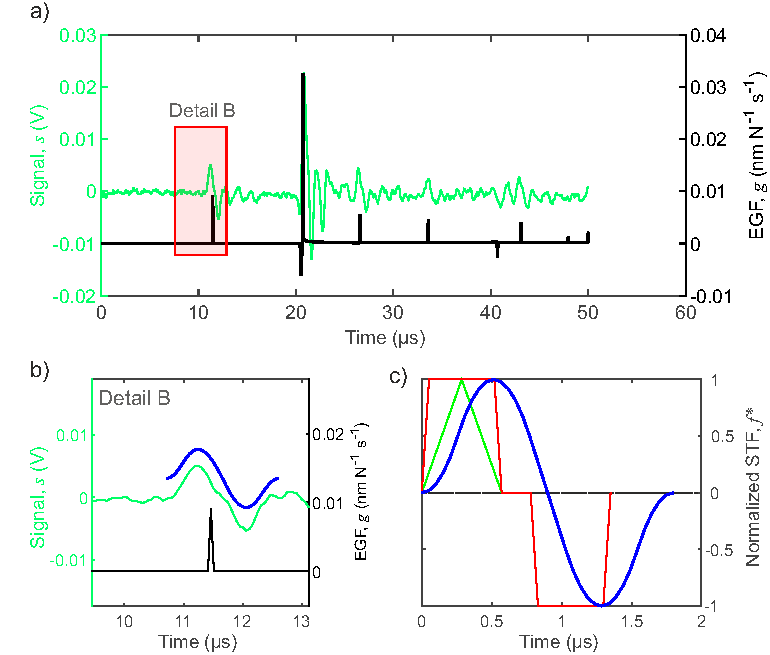
\includegraphics[scale= 1.0]{FIG6.pdf} 
\caption{Summary of the calibration experiments performed by \citet{Wu} to determine the instrument response for ball drops, performed \textit{a priori}, in the same location as where our PZT actuator was later placed. \textbf{(a)} The full range of calibrated frequencies (1 kHz to 1 MHz) is shown. \textbf{(b)} For our study, we only consider high-frequency aspect and therefore will only use the instrument responses between components 100 kHz to 1 MHz.  Colors are indicative of the sensors location as defined in Figure \ref{fig1}(b). For all the details please consult \citet{Wu}. }
	\label{fig6} 
\end{figure}

\subsection{Spectral Deconvolution}
\label{Spec_deconv}
Having the specific broadband instrument response, solved using the well-understood ball drop source for our exact sensor-source layout, is paramount to accurately model the force-time function of the PZT actuator described by equation \eqref{eq4b}.   If we now consider the original problem in Figure \ref{fig2}, we can start with the recorded signal produced from the PZT actuator and use the instrument response to determined the mechanical vibration.  In the Fourier domain, we can rearrange the left hand side of equation \eqref{eq3} to estimate the spectral response of the theoretical vibration $U_{k}(\mathbf{x},t)$ caused by the transient PZT actuator:

\begin{equation}
    \label{eq6}
\begin{split}
U_{k}\left( \mathbf{x}, \omega \right) & = 
        \frac{S\left( \mathbf{x}, \omega \right) }{ I_{k}\left( \mathbf{x},\omega \right)}.
\end{split}
\end{equation}

Approaching the problem from the source side (right hand side of equation \eqref{eq3}), we can estimate the mechanical vibration caused by the force of the PZT actuator convolved with the Green's function solution, which in the Fourier domain is shown as:

\begin{equation}
    \label{eq6a}
\begin{split}
U_{k}\left( \mathbf{x}, \omega \right) & = 
       F_{j}\left( \mathbf{\xi}, \omega \right)  \cdot G_{kj}\left(  \mathbf{x}, \omega; \mathbf{\xi}, \omega\right).
\end{split}
\end{equation}

\noindent Substituting the Fourier transform of the force-time function describe in equation \eqef{eq4}, we obtain

\begin{equation}
    \label{eq6b}
\begin{split}
U_{k}\left( \mathbf{x}, \omega \right) & = 
       A_{0}\cdot \delta (\omega)\cdot F^{*}_{j}\left( \mathbf{\xi}, \omega \right)  \cdot G_{kj}\left(  \mathbf{x}, \omega; \mathbf{\xi}, \omega\right),
\end{split}
\end{equation}

\noindent where the Fourier transform of the force-time magnitude parameter is $\mathcal{F}[A_{0}] = A_{0}\cdot\delta(\omega)$ and $\delta$ is the Dirac delta function.  Next we can combine equations \eqref{eq6} and \eqref{eq6b} to solve for the scaling factor for the force-time function $A_{0}$:


\begin{equation}
    \label{eq6c}
\begin{split}
 F_{j}\left( \mathbf{\xi}, \omega \right) = A_{0}\cdot \delta (\omega)  \cdot F^{*}_{j}\left( \mathbf{\xi}, \omega \right) & 
=\left[ \frac{S\left( \mathbf{x}, \omega \right) } 
{ I_{k}\left( \mathbf{x},\omega \right)} \right]
\left[ \frac{1}{ G_{kj}\left(  \mathbf{x}, \omega; \mathbf{\xi}, \omega\right)} \right].
\end{split}
\end{equation}

\noindent We see that all of the components on the right hand side can be measured ($S$), can be calculated ($G_{kj}$) or have been determined \textit{a priori} ($I_{k}$) . In this approach we assume that $A_{0}$ is constant over time and and the force-time function $f(\mathbf{\xi}, \tau)$ described accurately by equation \eqref{eq4b}.



\section{Results}
\label{results}
\subsection{Time domain analysis}
To test for source repeatability, we looked a a sweep of 15 pulses of the PZT actuator were performed.  The source was highly repeatable in at the high-frequencies we investigated.  From the 13 tests, the Pearson correlation coefficient (PCC) was analysed with respected to the stacked mean. We found that the average PCC = 0.9646 $\pm$ 0.03 over all the sensors for the 50 $\mu s$ time window analysed. We believe this to be representative of a repeatable source with respect to waveform similarities. Our final results will take these deviations into consideration; however, for clarity the results shown in this Section will focus on a single actuator pulse to highlight the methodology described in equations \eqref{eq1} to \eqref{eq6b}.

\begin{figure}[ht]
     	\centering
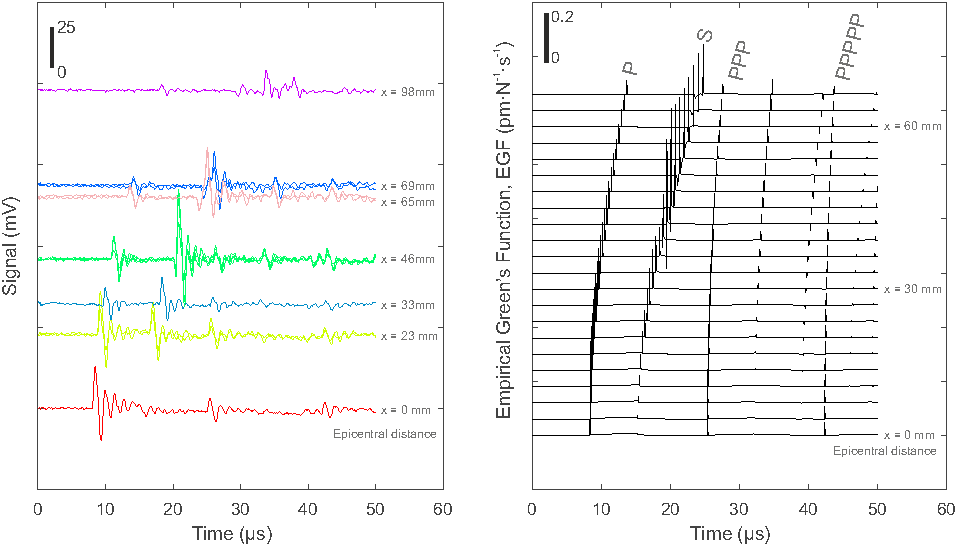
\includegraphics[scale= 1.0]{FIG3.pdf} 
\caption{\textbf{(a)} Measurements taken from the passive PZT transducers from a single transient PZT excitation described in Figure \ref{fig1}(d). The color scheme represents the different epicentral locations of each sensor in Figure \ref{fig1}(b).  \textbf{(b)} Green's function solutions determined using generalized ray theory for a semi-infinite elastic, homogeneous steel plate at different epicentral locations.  We see the various phase arrival predicted from the model.}
	\label{fig3} 
\end{figure}

In Figure \ref{fig3}(a) we show measurements on all passive sensors PZT sensors depicted in Figure \ref{fig1}(b) for a random pulse with color indicating different epicentral distances. For our analysis, we only the first 50 $\mu$s of signal since we do not want to pollute the data with reflections from the boundary of the platen that would occur if longer signals were analyzed. The sampling rate was $F_{s}$ = 20 MHz. Since boundary reflections are not considered, we can approximate that the plate is in fact semi-infinite. Under this assumption we are able to solve for the Green's functions using the generalized ray theory code provided by \citet{Hsu1985} and modified for MATLAB by \citet{McLaskey2012}.  Figure \ref{fig3}(b) shows the Green's functions at different epicentral locations, moving out from the source at $x$ = 0 mm. We call these approximations the empirical Green's function (EGF) since it is a numerical approximation of the true Green's function.  The true Green's function can be calculated by replacing the force-time function in equatoin \eqref{eq1} with the a unit impulse (Dirac delta) function $\delta_{j}(\mathbf{\xi}, \tau)$. In Figure \ref{fig3}(b) we also show the wave phase arrivals (P, S, PPP, PPPPP) from the numerical models.

\begin{figure}[ht]
     	\centering
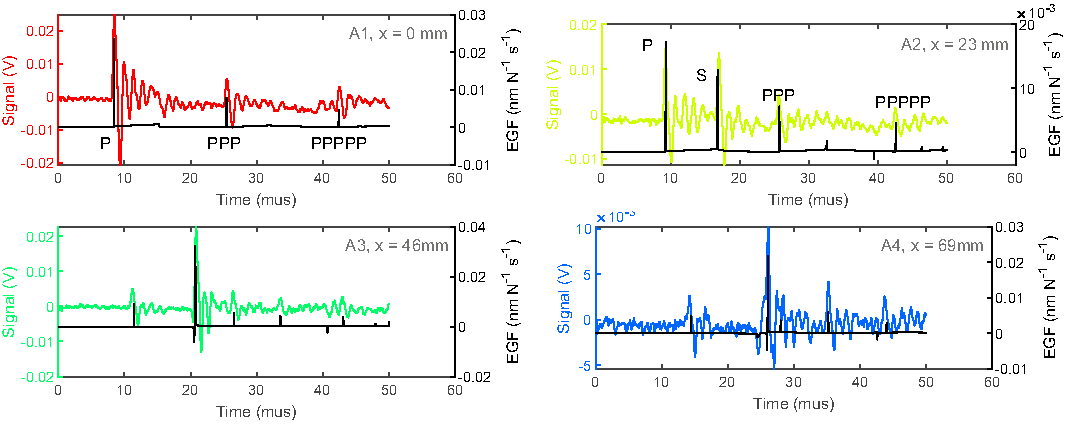
\includegraphics[scale= 0.90]{FIG4.pdf} 
\caption{Comparison of measurements on sensors A1, A2, A3 and A4 to the emipircal Green's functions calculated using generalized ray theory. The KRNBB sensor perform well and capture the wide range of wave phase arrivals.}
	\label{fig4} 
\end{figure}

Figure \ref{fig4} compares the theoretical Green's function $g_{kj}$ to the measured signals $s$.  For clarity, we only show the sensors A1 (red), A2 (yellow), A3 (green) and A4 (blue) at epicentral distances of 0 mm, 23 mm, 46 mm and 69 mm, respectively. We see that the sensors captures various phase arrivals predicted form the model. The ability of these sensors to accurately capture wave arrivals and information even at high azimuthal incident angles has been discussed in the literature \citep{Goodfellow2015, Selvadurai2019} and is due to the conical geometry of the PZT crystal. 

\begin{figure}[ht]
     	\centering
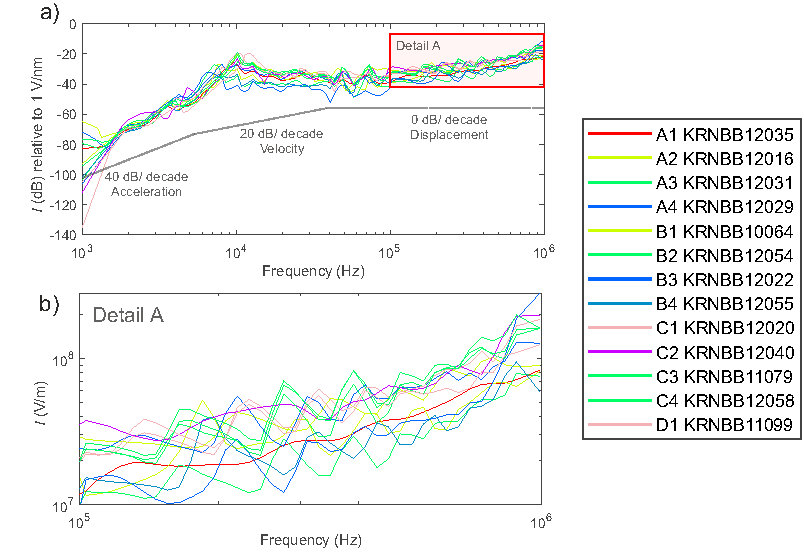
\includegraphics[scale= 0.85]{FIG5.pdf} 
\caption{\textbf{(a)} Measurements from sensor A3 (green line) from the active source compared to the EGFs at the same place from the model.  Detail B looks more closely at the first-arrival P wave. \textbf{(b)} Shows the general shape of the P wave (green line) versus the location of the expected P wave arrival (black line) form the Green's function solution.  From the convolutional nature of the wave propagation problem (equation \eqref{eq1}) we can estimate the general shape of the normalized force-time function $f^{*}_{j}$ shown as the blue line.}
	\label{fig5} 
\end{figure}

We further focus on the measurements taken from sensors A3 at epicentral distance $x$ = 46 mm. Figure \ref{fig5}(a) shows the measurements (green) and EGF (black line).  Detail B in Figure \ref{fig5}(b) focuses on the first arrival P wave. As discussed in Section \ref{force_time}, the measured waveforms will display features of the source due to the convolution operations in equations \eqref{eq1} to \eqref{eq3}. In Detail B we superimpose the normalized force-time function $f^{*}$ from Figure \ref{fig2b}(d) for reference. We see that there appears to be some similarities in our measured signals that would justify our hypothesized force-time function given in equation \eqref{eq4b}.  While the fit is not perfect -- the signal sensor A3 appears to a lower decay parameter $\Gamma$ -- this will be addressed when we simultaneously invert to match these variables on all sensors. Before doing so, we must calculate the scaling factor in the frequency domain using equation \eqref{eq6c}.

\subsection{Frequency domain analysis}
In this section we perform the discrete Fourier transform of the measured and theoretical traces in Figure \ref{fig3}.  For clarity we only show the results from the sensor A3 shown in Figure \ref{fig5} to illustrate the steps taken to solve for the scaling function $A_{0}$. To minimize the uncertainty that can occur from non-uniform spacing of samples of the Fourier frequencies linear scale, we average over multiple bins while evenly spacing our samples on the logarithmic scale.  We re-sample all DFT on the with 41 samples from 100 kHz to 1000 kHz.  While this might cause some averaging uncertainties between neighboring frequencies, this does not affect our final estimates of the scaling factor  $A_{0}$ in equation \eqref{eq6c} since, as we will see, we take estimate the scaling factor $A_{0}$ as a single average over the full range of frequencies. 

\begin{figure}[ht]
     	\centering
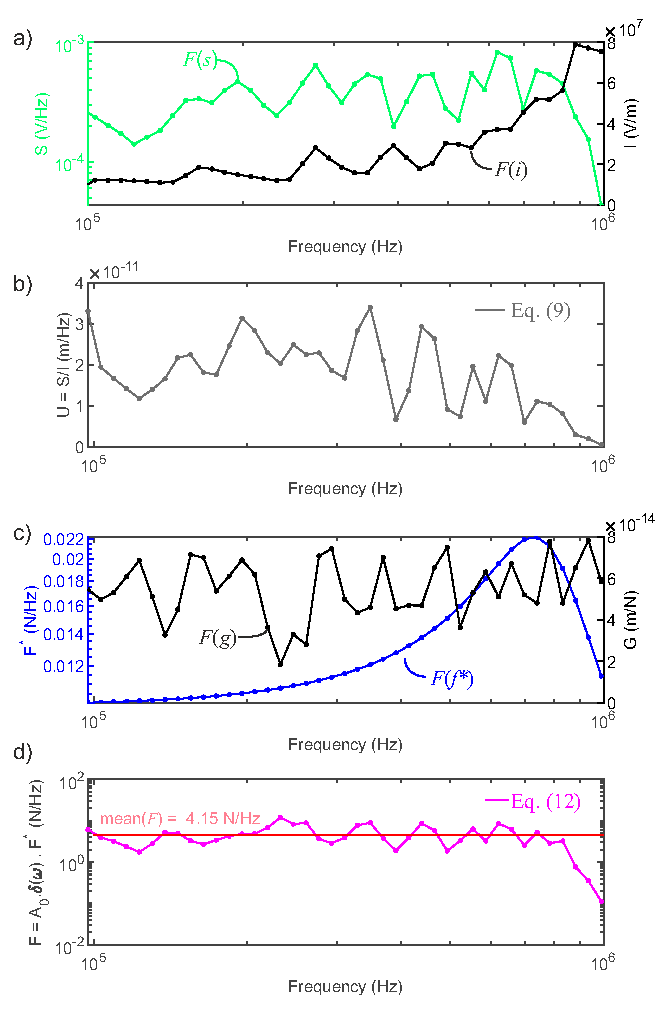
\includegraphics[scale= 0.9]{FIG7.pdf} 
\caption{\textbf{(a)} Discrete Fourier transform (DFT) of the measured waveform $S$ (green line) and the instrument response from sensor $I_{k}$ (black line) at A3 between 100 kHz to 1000 kHz. \textbf{(b)} Spectral estimates of the ground displacements $U_{k}$ (gray line) obtained from spectral division using equation \eqref{eq6}. \textbf{(c)} We show the DFT of the normalized force-time function $F_{j}^{*}$ (blue line) and the empirical Green's function $G_{kj}$ (black line) . \textbf{(d)} Spectral estimates of the corrected force time function $F$ calculated from the spectral estimates of the signal, instrument response, Green's function, normalized force time function. The spectral mean from between 100 kHz to 1000 kHz is shown.}
	\label{fig7} 
\end{figure}

Figure \ref{fig7}(a) shows the Fourier transform of the signal ($\mathcal{F}[s] = S$, green line) and instrument response ($\mathcal{F}[i] = I_{k}$, black line) for sensor A3 between frequencies from 100 kHz to 1000 kHz. Figure \ref{fig7}(b) shows spectral estimates of the theoretical ground motions $S$ from the signal side, i.e. from equation \eqref{eq6}.  As discussed in Section \label{Spec_deconv}, we can also try to estimate  theoretical ground motions from the source side.  Figure \ref{fig7}(c) shows the DFT of the empirical Green's function ($\mathcal{F}[g_{kj}] = G_{kj}$, black line) and the normalized force-time function ($\mathcal{F}[f^{*}_{j}] = F^{*}_{j}$, blue line). Figure \ref{fig7}(d), shows the spectral estimates of $F_{j}$ determined from using the previous results with equation \eqref{eq6c}.  The spectral response is relatively flat with a mean value of 3.4 N/Hz for our analysis on sensor A3.  Using the same approach on all other passive sensors we see an average 3.3 N/Hz with a standard deviation of 0.66 N/Hz. 

Using the calculations highlighted in Figure \ref{fig7}, we use the inverse Discrete Fourier transform (IDFT) to return the force-time function into the time domain. Firstly, due to the fact that the frequency response is relatively flat over the 100 kHz to 1000 kHz range (Figure \ref{fig7}(d)) we use the mean spectral value to scale the spectrum of normalized force-time function $F^{*}$ (blue line in Figure \ref{fig7}(c)) prior to performing the IDFT. We choose to scale the normalized source time function since, due to properties of the IDFT, we require frequencies outside the range we are able to estimate the spectral calculations shown in Figure \ref{fig7}.  We note that lower frequencies cannot be studied due to the plate finite geometry that limits our analysis of the signal to 50 $\mu s$.  

Figure \ref{fig9}(a) shows the all Fourier frequencies of our synthetic normalized force-time function $F^{*}$ from 20 kHz to 5 MHz (blue). Using the scaling factor from Figure \ref{fig7}(d), we can adjust our estimates that corrects our force-time function $F$ (black line) with calibration estimates from the instrument response determined form the ball drop. We have also applied a 4-pole bandpass butterworth filter $filt(F)$ (red line) between 100 kHz and 1000 kHz, which will be used in our time domain comparison between synthetic estimates to the filtered and unfiltered signals. Figure \ref{fig9}(b) shows the IDFT to our estimates of the normalized (blue), unfiltered (black) and filtered (red) force-time functions.  The corrected force-time function (black) in the time domain estimates that the peak force of $\sim$ 3.4 N. 

\begin{figure}[ht]
     	\centering
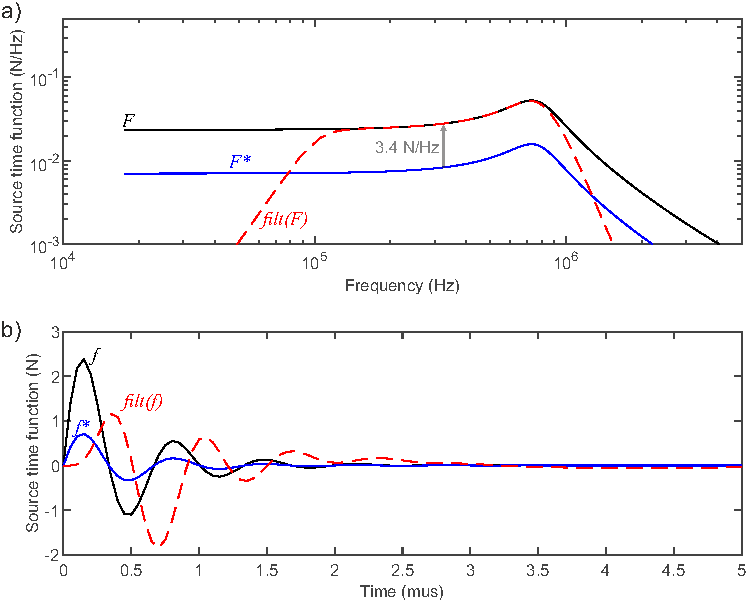
\includegraphics[scale=0.9]{FIG9.pdf} 
\caption{\textbf{(a)} Discrete Fourier transform (DFT) of the normalized $F^{*}$ (blue line), scaled $F$ (black line) and bandpass filtered $filt(F)$ (red line) of the force time function shown in Figure \ref{fig2b}(d). We show scaling factor of 3.4 N/Hz determined from the spectral analysis. \textbf{(b)} Inverse discrete Fourier transform (IDFT) of the signals in (a). }
	\label{fig9} 
\end{figure}
\subsection{Effects of receiver location on force-time estimates}

To better asses the variations in our estimates of $A_{0}$ with the spatial locations of the receivers we looked at results from all sensors for the 15 pulses. Figure \ref{fig9a}(a) shows the estimates of $A_{0}$ with takeoff angle $\theta$. The takeoff angle for this setup is depicted in Figure \ref{fig2}.  Piezoelectric transducers used in the laboratory have been known to be sensitive to incident angle of the incoming waves \citep{Goodfellow2015}.  This is also seen at the mining scale scale \citep{Kwaitek2011}. We see that there is a slight decrease in estimates of $A_{0}$ with increasing  $\theta$, with an average value of 2.3 N.  

Figure \ref{fig9a}(b) looks at dependence of $A_{0}$ on the total distance travelled (hypocentral distance).  Attenuation is the intrinsic loss in energy associated with a cycle of the wave for example by the internal friction of the material.  By fitting an exponential decay curve we can estimate the materials quality factor $Q$ -- a metric to describe the losses per cycle.  Our fit finds $A^{*}$ = 4.7 N and $\alpha$ = 0.01. Using these parameters we found the average $Q$ = 20,470 between 100 kHz to 1000 kHz, which is acceptable for steel (see Supplemental S2 for more details). It is impossible to perfectly determine whether the loss of sensitivity is related to the material property ($Q$) or a sensor characteristics due to the linear dependency of the hypocentral distance on $\theta$, however; material attenuation can explain this decrease with some degree of certainty. Taking into account attenuation, the value of the force at the source was $A^{*}$ = 4.7 N. This estimate falls within a reasonable range of estimated force-time function for conical sensor by \citet{Breckenridge1990} $\sim $ 1.2 N for a transient step function over 1 $\mu s$ with an amplitude of 100 V. If the systems studied by \citet{Breckenridge1990} was linear, we expect that 200 V we would result in a 2.4 N step.  This discrepancy may results from properties of the system (PZT geometry, casing, backing mass, damping material, electronics, data acquisition system, etc.), which is not identical to our making it difficult to perfectly characterize why they differ discrepancies. Moreover, the voltage-time function that excited the PZT actuator differs in each study; we employ a pulse-discharge excitation, whereas they employed a step-hold. However, we feel that the similarity in the order of $A_{0}$ is a positive results. 

\begin{figure}[ht]
     	\centering
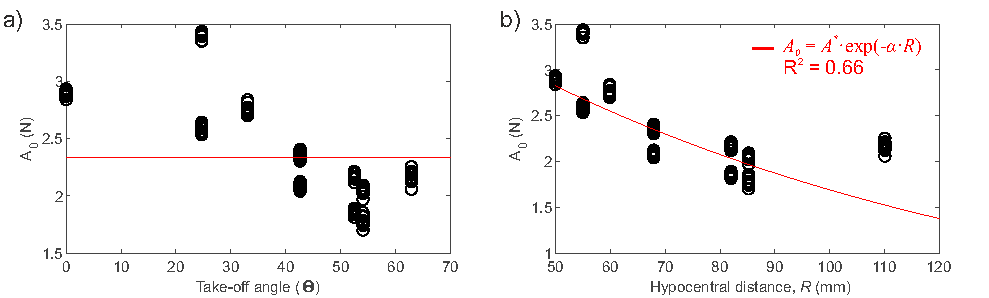
\includegraphics[scale= 1]{FIG9a.pdf} 
\caption{Relationships between spectral estimates of $A_{0}$ and the \textbf{(a)} takeoff angle ($\theta$) and \textbf{(b)} hypocentral distance ($R$). An exponential fit was used to determine the quality factor $Q$ (see Supplemental Section S2 for more details)  }
	\label{fig9a} 
\end{figure}
\subsection{Synthetic reconstructing}
Figure \ref{fig10} shows a comparison of the theoretical ground displacements for the estimated (a) unfiltered and (b) bandpass filtered force-time functions from Figure \ref{fig9}(b).  To calculate the theoretical displacements we convolve the force-time function with the Green's function following equation \eqref{eq2}. We see that the theoretical vibrations match the theory quite we on all sensors. This further enforces our hypothesis that the decrease in force estimates on sensors at higher takeoff angles was not a sensor sensitive issue but due to material attenuation. Figure \ref{fig10} is a rewarding result from this study and highlights the potential fully understanding the force-time function produced by our PZT actuator and HVP unit.  

\begin{figure}[ht]
     	\centering
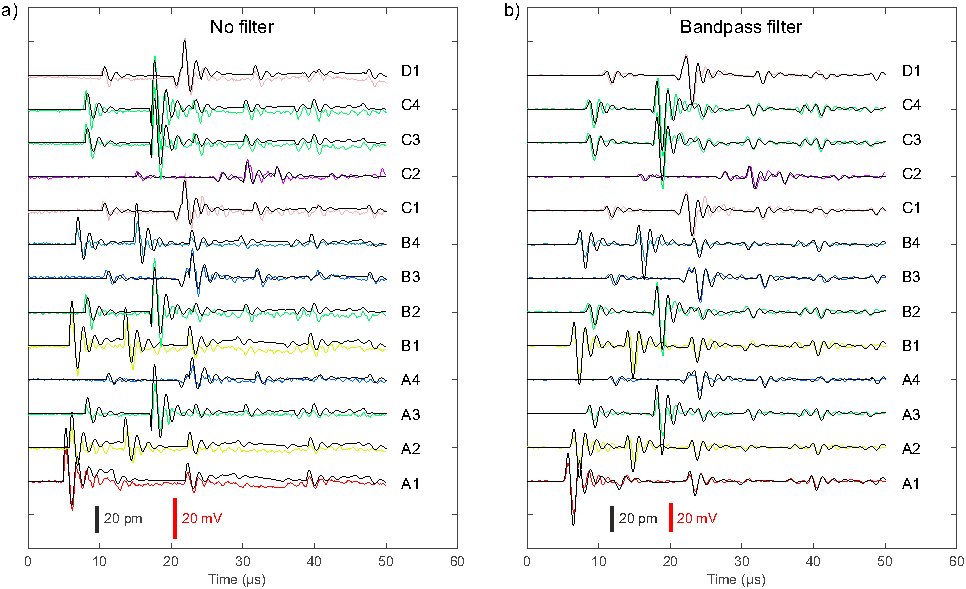
\includegraphics[scale= 1]{FIG10.pdf} 
\caption{\textbf{(a)}  }
	\label{fig10} 
\end{figure}

\section{Discussion}

Will complete later.  The discussion in this type of study is not that important I believe.

\textcolor{red}{The hope is to adopt techniques that have widely been used in the field of exploration geophysics in novel laboratories acoustic emission studies. To our knowledge, the benefits seen at scale from applications such as \textit{controlled-source interferometry} have not been fully explored in the laboratory with fully calibrated PZT actuator sources. We also see potential benefits when studying changes acoustic transmissivity \citep{PyrakNolte1980} with more accurate and coupled models that the simple linear slip model \citep[LSM,][]{Kendall1957}.  By understanding how various waves will be produced by our sensor (P and S waves) we can potentially understand the spatial variability in $V_{P}/V_{S}$ ratios to a higher degree of certainty. We foresee that an accurate transient force-time functions of our PZT actuators will help to frequently and non-invasively update time-dependent characteristics of the acoustic emission system component, such as: changes in passive transducer responses, in the transfer media or more accurate characteristics of similarly doublet events.} 

\section{Conclusions}
We have followed the recently popularized methodology for sensor calibration coupled reasonable understanding of the wave propagation problem in a semi-infinite, homogeneous elastic half space. By fully characterizing the individual components of our system, we show that it is possible to better understand the force-produced by a conical PZT actuator when excited by a rapid high-voltage transient. While the results presented here are unique to our system, the methodology and insight into the characteristic shape of the force-time function can be easily reproduced in other acoustic emission system. Fully understanding how system responses change during an experiment is critical to properly interpret seismicity in a quantitative manner. Our approach for time-dependent updates to calibration parameters but also can provide intrinsic and quantitative understanding of changes in the transfer media.

\section*{Acknowledgement}
The authors are indebted to the work and enthusiasm of Mr. T. M\"orgeli. He has been instrumental in the development of the infrastructure and provided critical input, design strategy and workmanship for the PZT actuator and the calibration station. His work is supported through the Rock Physics and Mechanics Laboratory at ETH Zurich.

Mr. Wu has been supported financially by China Scholarship Council (CSC, No. 201806440037). 

Dr. Selvadurai has was funded under FILL IN ASK STEFAN. 

Dr. Madonna was funded ...

Dr. Moradian was funded ...
 

\bibliographystyle{elsarticle-harv} 
\bibliography{Source_reconstruction}

\clearpage
\section*{Supplemental information}

\*subsection{Material Properties of PZT-5A (Navy II) }
\begin{table}[ht]
	\centering
	\caption{Material properties of Piezoelectric active source (PZT-5A).}
	\begin{tabular}{ m{5cm} m{2cm} m{4cm}} 
		\hline  
		\bf{Parameter} 		      & \bf{Symbol} 	  & \bf{Value}	\\
	   & \textit{Mechanical properties} & \\
	    Density                   & $\rho$            & 7500 kg/m$^{3}$\\
	    Poisson's ratio           & $\nu$             & 0.31\\
	    Young's modulus           & $E$               & 66 GPa\\
        Curie Point               & $T_{c}$           & 350 $^{o}$C\\  
        Mechanical quality factor &   $Q_{m}$         & 100\\
	  & \textit{Piezoelectric constants} & \\
 	  & d_{33}                   & 3.74 $\times$ 10$^{-10}$ m/V\\
 	  & d_{31}                   & -1.71 $\times$ 10$^{-10}$ m/V\\
	  & \textit{Dielectric constants} & \\
 	  & d_{33}                   & 3.74 $\times$ 10$^{-10}$ m/V\\
 	  & d_{31}                   & -1.71 $\times$ 10$^{-10}$ m/V\\

	       
		\hline  	
	\end{tabular}
	\label{table1}
\end{table}

\clearpage
\subsection*{S2 Quality Factor}
We estimate the quality factor in steel $Q_{steel}$ from estimates of the force magnitude $A_{0}$ at different hypocentral distances. This follow typical theory on attenuation used to model the damping of seismic waves over distance due to internal intrinsic losses (e.g. friciton) in the material that decreased the energy per cycle\citep[e.g.][]{Barton2007}. From Figure \ref{fig9}(b) we have fit the exponential decay over distance with $A^{*}$ = 4.7 N and $\alpha$ = 0.01 m$^{-1}$. The quality factor depends on the frequencies of the propagating wave and can be expressed as a function as follows

\begin{equation}
    \label{eqS2}
Q = \frac{\pi f}{V_{P}\alpha}.
\end{equation}

\noindent We can plot the quality factor over the frequency range 100 kHz to 1 MHz investigated in this study for $\alpha$ = 0.01 m$^{-1}$. Typical values of $Q_{steel} > $ 10,000 in the literature \citep{WaitingRUI}. Figure \ref{figS1} shows that at $f$ =100 kHz $Q$ = 5193, a relatively low estimate, and at $f$ = 1 MHz $Q$ = 51,935, which is a higher estimate for steel. Assume a constant attenuation quality factor of the range of 100 kHz to 1 MHz we obtain a average $Q$ = 20,470. 


\begin{figure}[ht]
     	\centering
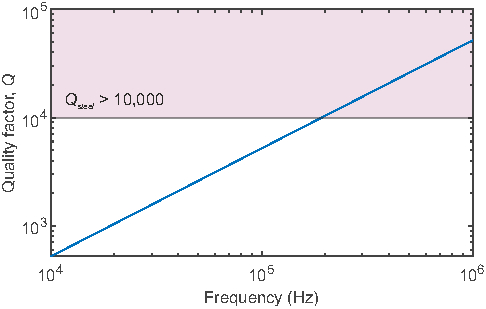
\includegraphics[scale= 1]{FIGS1.pdf} 
\caption{\textbf{(a)}  }
	\label{figS1} 
\end{figure}


\end{document}

\endinput
